\chapter{Enhancing the GUI}

In this chapter we'll add a dashboard to our app, including
\begin{itemize}
  \item a \emph{timer} for keeping track of the player's thinking time
  \item an indicator for \emph{material evaluation}
  \item the display of \emph{captured pieces} for each player
  \item a \emph{move indicator} for the last move
  \item a display for the complete \emph{moves history}, and
  \item an \emph{info field} for displaying messages from the app.
\end{itemize}

We will also store the current game to a textfile for later use, and add a splash-screen,
allowing to display the result of a game and to switch the game mode.

Furthermore, we will give a player the option to take back a move, to offer a draw,
and to resign.

Finally, we'll revisit some \emph{special moves}.

With all that in place, our app will look like so:

\begin{center}
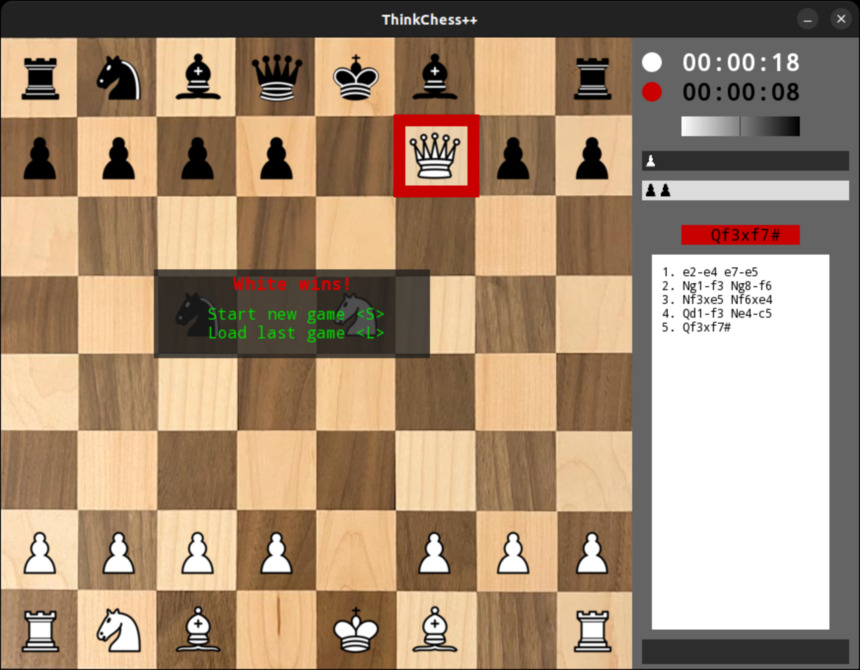
\includegraphics[width=\linewidth]{img/display.jpg}
\end{center}

\section{Refactoring}

First of all, I created a new translation unit at \texttt{app/display.cpp} and its
header file at \texttt{include/display.hpp}, which will contain all the display-oriented logic.

Next, I created another new unit at \texttt{app/position.cpp} and its header file at\\
\texttt{include/position.hpp} which contains all the move-oriented logic.\\
I moved all the functions from the old file \texttt{app/moves.cpp} to this new file and
deleted the old file.

This new file contains a new type \texttt{Position}, which holds all the position-relevant variables,
so I could delete those from the \texttt{main()} function.

\begin{cpp}
class Position {
public:
  ~Position() {}
  Position(short gs) : gamestate{gs}, player{true},
               board{8, vector<Piece*>(8)},
               mvCount{0}, castled{0}, checkmate{-1, -1},
               checked{false}, eval{0.f}
  {}

  // returns a material evaluation for both players
  void evaluate();

  // take back last move
  bool takeBackMove();

  // make a move
  bool makeMove(pair<int, int> from, pair<int, int> to);

  // gamestate: 0 = game over, 1 = 2-player, 2 = analyze 
  short gamestate;

  // player on turn, starting with white
  bool player;
  
  // matrix of pieces representing the board
  vector<vector<Piece*>> board;

  // vector of moves, used as a stack
  vector<string> moves;

  // list of captured pieces, used as a stack
  vector<Piece*> captured;

  // total count of moves
  int mvCount;
  
  // castled: 0 = no, 1 = white, 2 = black, 3 = both
  short castled;
  
  // coordinates of the piece, which gave checkmate
  std::pair<int, int> checkmate;
  
  // last move gave check
  bool checked;

  // basic evaluation of positions
  float eval;

  // infotext
  string info;
};
\end{cpp}

Observe, that I've made all the member types public, in order to avoid creating all the associated
\emph{getter} and \emph{setter} functions.
This would not be a good design decision, if we were to create a library, which was intended to
be used by different clients, as those clients could harm the game logic.
But, in our case, the only client is the \texttt{main()} function of our app, and I suppose that
we know what we are doing.

With the new type \texttt{Position} in place, we can initialize all relevant variables with a single
call from inside the main function: \mintinline{cpp}{Position position(0);} and call the
\texttt{makeMove} function with just two parameters (which are the field coordinates from the board)
like so: \mintinline{cpp}{position.makeMove(touched, to)}.

Finally, I extended the viewport of the app and made it not resizable:

\begin{cpp}
auto window = sf::RenderWindow{ {870, 640u},
                                "ThinkChess++",
                                sf::Style::Close,
                                settings };

window.clear(sf::Color(100, 100, 100));
\end{cpp}

The last line just sets the background of the display area to gray (inside the game loop).

\section{Timer}

For displaying the \emph{timer}, we first have to include the \texttt{chrono} library
and define two time counters, as well as two time points:

\begin{cpp}
#include <chrono>
using namespace chrono;

unsigned wTime = 0;
unsigned bTime = 0;
steady_clock::time_point last;
last = steady_clock::now();
steady_clock::time_point now;
\end{cpp}

For calculating the current thinking time for both player, we have this code inside the
game loop, just before drawing anything:

\begin{cpp*}{linenos}
if (position.gamestate == 1) {
  now = steady_clock::now();
  if (now - last > 1s) {
    last = steady_clock::now();
    if (position.player) wTime++;
    else bTime++;
  }
}
\end{cpp*}

The code checks, wether we are in playing mode (gamestate is set to 1), and captures the current
time point (2).
If the difference between \texttt{now} and \texttt{last} is greater than one second (3), increase
the time counter for the player whose turn it is (5-6).
Remember, we have set the \texttt{sf::FramerateLimit} to 10, so this code will be called 10 times
pers second, and we cannot simply increase the time counters for each pass.

In oder to actually draw the timer, we have this code inside the game loop (directly after the
last code snippet):

\begin{cpp*}{linenos}
string timer = "";
if (position.player) {
  window.draw(wActive);
  timer = getTime(wTime);
  wTimer.setString(timer);
} else {
  window.draw(bActive);
  timer = getTime(bTime);
  bTimer.setString(timer);
}
if (position.checkmate.first != -1) {
  if (position.player) {
    bActive.setFillColor(sf::Color(200, 0, 0));
    window.draw(bActive);
  } else {
    wActive.setFillColor(sf::Color(200, 0, 0));
    window.draw(wActive);
  }
}
window.draw(wTimer);
window.draw(bTimer);
\end{cpp*}

This code also draws the indicator for the active player (the white or black circle in front of
the timer) in lines 3 and 7.
If the app has detected a checkmate (11), the active player's indicator is set to a red color
(13, 16).

For that to work, we need to have the respective \texttt{sf::Sprite}s to be defined (before
entering the game loop):

\begin{cpp*}{linenos}
// set timer
sf::Text wTimer;
wTimer.setFont(noto);
wTimer.setCharacterSize(24);
wTimer.setStyle(sf::Text::Bold);
wTimer.setFillColor(sf::Color::White);
wTimer.setString("00:00:00");
wTimer.setPosition(690.f, 10.f);

sf::Text bTimer = wTimer;
bTimer.setFillColor(sf::Color::Black);
bTimer.setPosition(690.f, 40.f);

// marker for aktive player
sf::CircleShape wActive(10.f);
wActive.setPosition(650.f, 15.f);
wActive.setFillColor(sf::Color::White);

sf::CircleShape bActive(10.f);
bActive.setPosition(650.f, 45.f);
bActive.setFillColor(sf::Color::Black);
\end{cpp*}

In order to display text with SFML, we have to set a font to the \texttt{sf::Text} sprite (3),
and we also must have a font already in place (just before the last snippet):

\begin{cpp}
sf::Font noto;
if (!noto.loadFromFile("../img/NotoMono-Regular.ttf")) {
  cout << "failed to load the font\n";
  return 1;
}
\end{cpp}

I have chosen the \emph{NotoMono-Regular} font, because it is a fixed-space font and quite compact:
it only contains 897 glyphs (the images for actually drawing each character), in contrast to
more than 5,000 glyphs for fancier fonts.

The last thing missing is the function \texttt{getTime()} to convert a time counter (an unsigned
integer value) into a readable time format. This function is located inside the new
\texttt{app/display.cpp} implementation file:

\begin{cpp*}{linenos}
string getTime(unsigned t) {
  string result = "";
  unsigned h = 0;
  unsigned m = t / 60;
  unsigned s = t % 60;
  if (m >= 60) {
    h = m / 60;
    m = m % 60;
  }
  if (h < 10) {
    result.append(1, '0');
    result.append(to_string(h));
  } else {
    result.append(to_string(h));
  }
  result.append(1, ':');
  if (m < 10) {
    result.append(1, '0');
    result.append(to_string(m));
  } else {
    result.append(to_string(m));
  }
  result.append(1, ':');
  if (s < 10) {
    result.append(1, '0');
    result.append(to_string(s));
  } else {
    result.append(to_string(s));
  }
  return result;
}
\end{cpp*}

The logic is straight forward: just divide the total amount of seconds by 60 to get the minutes (4),
and take the ramainder of that calculation to get the remaining seconds (5).
If the resulting minutes are greater than 60 (6), repeat those steps to get the hours and remaining
minutes (7-8).
The rest of the code (10-29) is just for formatting: if hours, minutes, and seconds are less than 10,
insert the digit \texttt{0}  at the appropriate position.

\section{Material evaluation}

\emph{Material evaluation} is the first step in evaluating the players positions on the board.

Evaluating positions is a copmlex task, for which one must have a deeper understanding of
several factors, including the pawn structure, control of the center, space and initiative.
We'll explore the basics of position evaluation in the next chapter, which will also be the first
chapter mainly about \emph{playing} chess.

For now, we are only interested in the first part of this process, which is straight forward:
add up the values of the pieces of each player and compare them.

For that we need a new function, which needs access to the board; so it's
a natural choice to define it as a member of the type \texttt{Position}:

\begin{cpp}
void evaluate() {
  pair<int, int> matEval = evaluateBoard(board);
  eval = float(matEval.first) / 100
       - float(matEval.second) / 100;
}
\end{cpp}

The function calls a helper function, which is defined in the corresponding implementation file:

\begin{cpp}
pair<int, int> evaluateBoard(const vector<vector<Piece*>>& bd) {
  int white = 0;
  int black = 0;
  
  for (int row = 0; row < 8; row++) {
    for (int col = 0; col < 8; col++) {
      auto pc = bd[row][col];
      if (pc) {
        pc->isWhite() ? white += pc->getValue()
                      : black += pc->getValue();
      }
    }
  }
  pair<int, int> eval = make_pair(white, black);
  return eval;
}
\end{cpp}

Observe my design choice: I defined all functions, which need a reference to the board, but
will not modify it, as helper functions outside the class \texttt{Position}, and I made the
reference to the board \mintinline{cpp}{const}. So the compiler will ensure that indeed
no updates to the board will happen inside those functions.

I also decided to sligthly modify the value scheme for pieces of section~\ref{subsec:pieces}:
the queen now has a value of 9, and the rooks each a value of 5.
To be able to do more accurate calculations later, the values are defined as \emph{centipawns}
by multiplying them with 100.
With that, we'll be able to make all future calculations on the base of integer values,
which should be faster than calculating with \mintinline{cpp}{float} representations of the
value.

The current implementations of the pieces look like so:

\begin{cpp}
class Queen : public Piece {
public:
  ~Queen() {}
  Queen(bool w, int r, int c) :
    type{'Q'}, white{w}, value{900}, row{r}, col{c} {}

  char getType() override { return type; }
  int getValue() override { return value; }
  bool isWhite() override { return white; }
  int getRow() override { return row; }
  int getCol() override { return col; }
  void makeMove(int r, int c) override { row = r; col = c; }
  bool isValid(const vector<vector<Piece*>>& bd, int r, int c) override;

private:
  char type;
  bool white;
  int value;
  int row;
  int col;
};
\end{cpp}

Now we can use the evaluation function inside the game loop to actually draw the
\emph{evaluation meter}:

\begin{cpp*}{linenos}
if (moved) {
  if (position.mvCount % 2 == 0) {
    position.evaluate();
    eval = position.eval;
    if (eval > 10.0) {
      eval = 10.f;
      mb[2].color = sf::Color(200, 0, 0, 200);
      mb[4].color = sf::Color(200, 0, 0, 200);
      mb[5].color = sf::Color(200, 0, 0, 200);
    }
    if (eval < -10.0) {
      eval = -10.f;
      mb[0].color = sf::Color(200, 0, 0, 200);
      mb[1].color = sf::Color(200, 0, 0, 200);
      mb[3].color = sf::Color(200, 0, 0, 200);
    }
    mi[2].position = sf::Vector2f(750.f + eval*6.f, 80.f);
    mi[3].position = sf::Vector2f(750.f + eval*6.f, 100.f);
    if (eval > 0) {
      mi[2].color = sf::Color::White;
      mi[3].color = sf::Color::White;
    } else {
      mi[2].color = sf::Color::Black;
      mi[3].color = sf::Color::Black;
    }
  }
}
\end{cpp*}

When a move is complete, i.e. both players have moved (2), evaluate the material (3).
Then, set the local variable \texttt{eval} to the calculated value (4);
we are doing so, because we don't want to tinker with the member variables of
\texttt{Position} from outside the class (remember my caveat for this design decision).\\
For display purposes, we restict that value to the range $[-10, 10]$, and set the
background color of the evaluation meter to red, if the value is outside
that range (5-16).\\
Finally, we set the position and the color of the evaluation indicator (17-24).
We'll see soon, how this works.

You may have noticed that this code will only be executed, if a move was made (1).
Remember, this code is placed inside the game loop, and we don't want to evaluate the board
for every update of the display.
So I modified the \mintinline{cpp}{Position::makeMove()} function to report success, and call
it like so: \mintinline{cpp}{moved = position.makeMove(touched, to)}:

\begin{cpp}
bool makeMove(pair<int, int> td, pair<int, int> to) {
  auto pcf = board[td.first][td.second];
  auto pct = board[to.first][to.second];

  if (!pcf) {
    info = "no piece selected";
    return false;
  }
  if (pcf->isWhite() != player) {
    info = "it's not your turn";
    return false;
  }
  // --- snip ---
}
\end{cpp}

The background of the evaluation meter (\texttt{mb}) is defined as an SFML primitive
(a set of two unconnected triangles), and the evaluation indicator (\texttt{mi})
as a set of two unconnected vertical lines:

\begin{cpp*}{linenos}
sf::VertexArray mb(sf::Triangles, 6);
mb[0].position = sf::Vector2f(690.f, 80.f);
mb[1].position = sf::Vector2f(690.f, 100.f);
mb[2].position = sf::Vector2f(810.f, 100.f);
mb[3].position = sf::Vector2f(690.f, 80.f);
mb[4].position = sf::Vector2f(810.f, 80.f);
mb[5].position = sf::Vector2f(810.f, 100.f);
mb[0].color = sf::Color::White;
mb[1].color = sf::Color::White;
mb[2].color = sf::Color::Black;
mb[3].color = sf::Color::White;
mb[4].color = sf::Color::Black;
mb[5].color = sf::Color::Black;

sf::VertexArray mi(sf::Lines, 4);
mi[0].position = sf::Vector2f(750.f, 80.f);
mi[1].position = sf::Vector2f(750.f, 100.f);
mi[2].position = sf::Vector2f(750.f, 80.f);
mi[3].position = sf::Vector2f(750.f, 100.f);
mi[0].color = sf::Color::Green;
mi[1].color = sf::Color::Green;
mi[2].color = sf::Color::Black;
mi[3].color = sf::Color::Black;
\end{cpp*}

I've set the color of the triangle points to black and white, such that the meter's 
background color is interpolated to fill the background with a gradient from white to black.
The green line of the indicator shows the neutral position (the evaluation value 0) and it's
static.
The black line ($mi[2]$ and $mi[3]$) is the actual indicator, which we have
updated when processing a move.

With this setup, the indicator will move to the right when the evaluation value is greater than
zero (i.e. white has an advantage), and move to the left when black has an advantage.
This may seem counter-intuitive at first, but once you get used to it, you'll catch the
evaluation at a glance.

\section{Captured pieces}

For displaying the captured pieces of each player, we only need two background areas:

\begin{cpp}
sf::RectangleShape bcw(sf::Vector2f(210.f, 20.f));
bcw.setFillColor(sf::Color(30, 30, 30, 200));
bcw.setPosition(650.f, 115.f);
sf::RectangleShape bcb = bcw;
bcb.setFillColor(sf::Color(220, 220, 220));
bcb.move(0.f, 30.f);
\end{cpp}

and a way to draw miniature versions of the pieces figures onto those:

\begin{cpp}
window.draw(bcw);
window.draw(bcb);
int wc = -1;
int bc = -1;
for (auto piece : position.captured) {
  sf::Sprite cp;
  switch (piece->getType()) {
  case 'K':
    piece->isWhite() ? cp = wk : cp = bk;
    break;
  case 'Q':
    piece->isWhite() ? cp = wq : cp = bq;
    break;
  case 'R':
    piece->isWhite() ? cp = wr : cp = br;
    break;
  case 'B':
    piece->isWhite() ? cp = wb : cp = bb;
    break;
  case 'N':
    piece->isWhite() ? cp = wn : cp = bn;
    break;
  case 'P':
    piece->isWhite() ? cp = wp : cp = bp;
    break;
  }
  cp.scale(0.3f, 0.3f);
  if (piece->isWhite()) {
    wc++;
    cp.setPosition(650.f + wc*15.f, 115.f);
  } else {
    bc++;
    cp.setPosition(650.f + bc*15.f, 145.f);
  }
  window.draw(cp);
}
\end{cpp}

Getting the captured pieces is easy, as we had already stored them in a separate
data structure \texttt{captured} within the \texttt{position} object, while making a move:

\begin{cpp}
// valid move?
if (pcf->isValid(board, to.first, to.second)) {
  // can capture?
  if (pct && pct->isWhite() != pcf->isWhite()) {
    cap = true;
    captured.push_back(pct);
  } else if (pct) { // same color
    info = "illegal move";
    return false;
  }
  // --- snip ---
}
\end{cpp}

I've rejected the idea of storing the captures pieces in a linked list; instead, I'm using
a vector of pieces: \mintinline{cpp}{vector<Piece*>}.
We can easily use a vector as a \emph{stack} (a \emph{LIFO} data structure) by using its
member functions \mintinline{cpp}{push_back()} and \mintinline{cpp}{pop_back()}
in a very performant way.
Additionally, vectors provide an iterator, which we can use in the \emph{range-for} statement
\mintinline{cpp}{for (auto piece : position.captured)}, without actually \emph{popping} the
elements.

\section{Move indicator}

The \emph{move indicator} is implemented with a similar pattern:

\begin{cpp}
// current move background
sf::RectangleShape mvb(sf::Vector2f(120.f, 20.f));
mvb.setFillColor(sf::Color(200, 200, 0, 200));
mvb.setPosition(690.f, 190.f);

// current move indicator
sf::Text mvi;
mvi.setFont(noto);
mvi.setCharacterSize(16);
mvi.setFillColor(sf::Color::Black);
mvi.setPosition(720.f, 190.f);
\end{cpp}

As with the evaluation meter, we only update the move indicator when a move was made:

\begin{cpp}
if (moved) {
  // --- snip ---
  position.mvCount > 0 ? mvi.setString(position.moves.back())
                       : mvi.setString("");
  position.checked ? mvb.setFillColor(sf::Color(200, 100, 0, 200))
                   : mvb.setFillColor(sf::Color(200, 200, 0, 200));
  position.checked = false;
  position.info.clear();
  itt.setString("");
  // --- snip ---
}
\end{cpp}

Additionally, if the \mintinline{cpp}{position.checked} flag was set when making the move,
we set the background color of the move indicator to orange.

\section{Moves history}

The next feature of our GUI is the display of the complete moves history for a game,
but we also want to persintently store the hsitory in a text file.
This is done with the follwing code:

\begin{cpp*}{linenos}
if (moved) {
  // --- snip ---
  if (position.mvCount % 2 == 0) {
    game << position.moves.back() << "\n";
    history += position.moves.back();
    history += "\n";
  } else {
    game << (position.mvCount / 2) + 1 << ". "
         << position.moves.back() << " ";
    history += to_string((position.mvCount / 2) + 1);
    history += ". ";
    history += position.moves.back();
    history += " ";
  }
  // trim history string
  if (position.mvCount > 52 && position.mvCount % 2 == 1) { 
    auto pos = history.find("\n") + 1;
    history = history.substr(pos, history.size());
  }
  hist.setString(history);
  // --- snip ---
}
\end{cpp*}

If it was a black move (3), write the move in algebraic notation to the file-stream
\texttt{game} and add a newline (4).
Also add it to the \texttt{history} string (5-6).\\
If it was a white move (7), write it to the file-stream as well (9), but only after
prepending it with the current move number (8).
Also add the move to the history string (10-13).\\
If there are more than 52 half-moves (i.e. 26 complete moves) in the history (16),
we trim the history string from its beginning (17-18), as there's only space for
26 moves in the history display area.
But, we'll never trim the history of the file stream, so there's no action needed
in this case.

In order for this to work, we need to have the file-stream and the history field in place:

\begin{cpp}
#include <fstream>

string lastGame = "../games/last.txt";
std::fstream game;

// moves history
sf::RectangleShape hisb(sf::Vector2f(180.f, 380.f));
hisb.setFillColor(sf::Color::White);
hisb.setPosition(660.f, 220.f);
sf::Text hist;
hist.setFont(noto);
hist.setCharacterSize(12);
hist.setFillColor(sf::Color::Black);
hist.setPosition(670.f, 230.f);
\end{cpp}

We're using an \texttt{fstream} to be able to read from and write to that stream.
But that's not enough: we also need to make sure that the game file actually exists,
and if not, to create it:

\begin{cpp*}{linenos}
game.open(lastGame, std::ios::trunc);
if (!game.is_open()) {
  game.clear();
  game.open(lastGame, std::ios::out); // create file
  game.close();
  game.open(lastGame);
}
\end{cpp*}

If the file already exists, open it in truncation mode, so that all contents will
be cleared (1).
If not (2), re-open the file in output mode to create the file (4), close and open
it again in write mode (5-6).

We must not forget do synchronize the file stream with the actual file and to close the
stream whenever a game is finished:

\begin{cpp}
if (game.is_open()) {
  game.flush();
  game.close();
}
\end{cpp}

This is currently done in two cases: when the main window is closed (inside the event loop),
and when a checkmate is detected (at the very end of the game loop).

\section{Keyboard input}
\subsection{Splash Screen}

First, we're going to add a splash screen to our GUI to be able to start and end a game properly:

\begin{cpp}
sf::RectangleShape bsplash(sf::Vector2f(280.f, 90.f));
bsplash.setFillColor(sf::Color(30, 30, 30, 200));
bsplash.setPosition(155.f, 235.f);
sf::Text welcome;
welcome.setFont(noto);
welcome.setCharacterSize(16);
welcome.setFillColor(sf::Color(220, 0, 0));
welcome.setStyle(sf::Text::Bold);
welcome.setPosition(170.f, 240.f);
welcome.setString("Welcome to ThinkChess++");
sf::Text spt;
spt.setFont(noto);
spt.setCharacterSize(16);
spt.setFillColor(sf::Color(0, 220, 0));
spt.setPosition(210.f, 270.f);
spt.setString("Start new game <S>\nLoad last game <L>");
\end{cpp}

Remember, we initialize the main position object like so: \mintinline{cpp}{Position position(0);}\\
Having the gamestate initially set to 0, allows us to distinguish between the game modes and
to draw the display, when starting a new game, like so:

\begin{cpp}
// inside game loop
if (position.gamestate == 0) {
  window.draw(bsplash);
  window.draw(spt);
  if (position.checkmate.first != -1) {
    string restart;
    if (position.player) restart = "      White ";
    else restart = "      Black ";
    restart.append("wins!");
    welcome.setString(restart);
  }
  window.draw(welcome);
}
\end{cpp}

This also allows us to distinguish between modes inside the event loop, and the player is able
to start a new game in splash mode:

\begin{cpp*}{linenos}
// inside event loop
if (position.gamestate == 0) {
  if (sf::Keyboard::isKeyPressed(sf::Keyboard::S)) {
    position = Position(1);
    resetBoard(position);
    game.open(lastGame, std::ios::trunc);
    if (!game.is_open()) {
      game.clear();
      game.open(lastGame, std::ios::out); // create file
      game.close();
      game.open(lastGame);
    }
    bActive.setFillColor(sf::Color::Black);
    wActive.setFillColor(sf::Color::White);
    mi[2].position = sf::Vector2f(750.f - position.eval*3.f, 80.f);
    mi[3].position = sf::Vector2f(750.f - position.eval*3.f, 100.f);
    mvb.setFillColor(sf::Color(200, 200, 0, 200));
    mvi.setString("");
    wTime = 0;
    bTime = 0;
    last = chrono::steady_clock::now();
    bTimer.setString("00:00:00");
    history.clear();
    hist.setString(history);
  }
}
\end{cpp*}

Here, we read input from the keyboard (3) and if the key `S' is pressed, the position object
is re-created with gamestate 1 (4), and the board is reset (5).\\
We also re-load the game file (6-12, which we have seen in the last section),
and reset the active players indicators (13-14).\\
The evaluation meter is also reset (15-17) and the move indicator cleared (17-18).\\
Then, reset the thinking time for both players (19-20), start the timer (21) and
reset the timers display (22).
Finally, clear the moves history (23-24).

All this is necessary because of this: we use the splash screen not only when starting the app,
but also whenever a checkmate during a game is detected and the game is ended:

\begin{cpp}
// last statement in game loop
if (position.checkmate.first != -1) {
  position.gamestate = 0;
  if (game.is_open()) {
    if (position.player) {
      game << "\n";
      game << "1-0\n";
    }
    else game << "0-1\n";
    game.flush();
    game.close();
  }
}
\end{cpp}

\subsection{Draw and resign}

In section~\ref{subsec:stale} we learned that our app will not discover a \emph{stalemate}.
To make up for this, each player gets the opportunity to offer a draw, after a move has made.

\begin{cpp*}{linenos}
// inside event loop
if (position.gamestate == 1) {
  // draw offer
  if (sf::Keyboard::isKeyPressed(sf::Keyboard::D) && !draw) {
    draw = true;
    itt.setString("Accept a draw? (Y/N)");
  }
  // respond to draw offer
  if (sf::Keyboard::isKeyPressed(sf::Keyboard::Y) && draw) {
    position.gamestate = 0;
    draw = false;
    if (!position.player) game << "\n";
    game << "1/2-1/2\n";
    game.flush();
    game.close();
    welcome.setString("     It's a draw!");
  }
  if (sf::Keyboard::isKeyPressed(sf::Keyboard::N) && draw) {
    itt.setString("Draw offer declined.");
    draw = false;
  }
  // --- snip ---
}
\end{cpp*}

If the D-key is pressed during the game (4), a corresponding message is displayed (6).\\
Now the other player has to decide if she's accepting the draw.
If so, she'll respond with `Y' (9), and the game is ended (10) and the result is recorded (12-16).\\
Otherwise, if the response is `N' (18), the draw offer is declined (19) and the player, who
made the offer, is still on turn.

Observe that the app will only respond to the keys `Y' and `N', if a draw was actually offered,
in order to prevent unintentional draw (9, 18).

Similar rules are in place, when a player wants to resign:

\begin{cpp}
if (sf::Keyboard::isKeyPressed(sf::Keyboard::G) && !giveUp) {
  giveUp = true;
  itt.setString("Sure to give up? (Y/N)");
}
if (sf::Keyboard::isKeyPressed(sf::Keyboard::Y) && giveUp) {
  position.gamestate = 0;
  giveUp = false;
  if (position.player) {
    game << "0-1\n";
    welcome.setString("    White gives up!\n");
  } else {
    game << "\n";
    game << "1-0\n";
    welcome.setString("    Black gives up!\n");
  }
  game.flush();
  game.close();
}
if (sf::Keyboard::isKeyPressed(sf::Keyboard::N) && giveUp) {
  giveUp = false;
  itt.setString("Okay, move on.");
}
\end{cpp}

But this time, the player who made the request is expected to confirm, again in order to
prevent unintentional resign.

For both cases, draw and resign, the app will behave like this: if no answer is given to
the request, the player whose turn it is, can proceed with a regular move, and the request
is declined.

\subsection{Take back a move}


\section{Special moves revistited}

